\documentclass[12pt]{article}
 
\usepackage[margin=1in]{geometry}
\usepackage{amsmath,amsthm,amssymb,mathtools,amsfonts}
\usepackage{graphicx}
\usepackage{caption}
\usepackage{subcaption}
 
\newcommand{\N}{\mathbb{N}}
\newcommand{\R}{\mathbb{R}}
\newcommand{\Z}{\mathbb{Z}}
\newcommand{\Q}{\mathbb{Q}}
\newcommand{\C}{\mathbb{C}}
\newcommand{\defeq}{\vcentcolon=}
\newcommand{\eqdef}{=\vcentcolon}
\newcommand{\overbar}[1]{\mkern 1.5mu\overline{\mkern-1.5mu#1\mkern-1.5mu}\mkern 1.5mu}

\newenvironment{theorem}[2][Theorem]{\begin{trivlist}
\item[\hskip \labelsep {\bfseries #1}\hskip \labelsep {\bfseries #2.}]}{\end{trivlist}}
\newenvironment{lemma}[2][Lemma]{\begin{trivlist}
\item[\hskip \labelsep {\bfseries #1}\hskip \labelsep {\bfseries #2.}]}{\end{trivlist}}
\newenvironment{exercise}[2][Exercise]{\begin{trivlist}
\item[\hskip \labelsep {\bfseries #1}\hskip \labelsep {\bfseries #2.}]}{\end{trivlist}}
\newenvironment{problem}[2][Problem]{\begin{trivlist}
\item[\hskip \labelsep {\bfseries #1}\hskip \labelsep {\bfseries #2.}]}{\end{trivlist}}
\newenvironment{question}[2][Question]{\begin{trivlist}
\item[\hskip \labelsep {\bfseries #1}\hskip \labelsep {\bfseries #2.}]}{\end{trivlist}}
\newenvironment{corollary}[2][Corollary]{\begin{trivlist}
\item[\hskip \labelsep {\bfseries #1}\hskip \labelsep {\bfseries #2.}]}{\end{trivlist}}
 
\begin{document}
\title{CS 7646 Strategy Learner}
\author{Michael Groff \\ ID\# 902772277}
\maketitle
For this project the goal was to develop a machine learning algorithm to frame the problem of picking a stock and entering and exiting short and long positions to maximize the cumulative revenue over some time period. I chose to frame the problem with a q-learner by taking the price data of that stock and using 4 technical indicators to create different states and decided whether it would be more advantageous to buy, sell, or cash out. Taking the same four indicators used in the earlier Manual Strategy project: Simple Moving Average, Momentum, Bollinger Bands, and Fibonacci Retracement. Each of these indicators was discretized by first taking the difference in the charted values and the daily prices of the stock to obtain a smaller range with both positive and negative values, in the case of bollinger bands only the top band was used as it was expected that the learner would also be able to learn where the bottom band was since it would translate to a static distance from the top band, similarly with fibonacci retracement only the 61.8 was discretized as the best distances from this band to buy or sell should be capitalized on by our learner. Discretization was done by taking the most extreme value in each set extending the bounds slightly and splitting the difference into ten evenly spaced bins, a 4-tuple that identified which of these bins a certain days price would fall in for each of the indicators. As we had a set training period we framed this period as a single epoch and used the set state capability to determine the action for the first day and using that action kept track of the portfolio value in the exact same way as in the Manual Strategy (taking into account commission and impact with each sale). Using the change in the portfolio value into the next day/state this positive or negative value was used as the reward for the QLearner. I also chose not to utilize a non zero dyna for this learner as there was not much to be gained from experience replay as in each epoch we had no choice but to loop through the same set of states (albeit with different rewards depending on the action used right before). When using dyna in sample although a good Q learner was formed in less epochs the time cost rose high enough that there was very little difference in overall time and accuracy. \\
\text{ }\\
For the first experiment the q learner was trained using data from the stock JPM for January 1, 2008 to December 31 2009 with a starting cash value of \$100,000 a standard commision of 9.95 and impact value of 0.005 was used and the in sample results were compared as well as those out of the sample. The q learner performed extremely well with a normalized cumulative return of 1.978 and an average daily return of 0.0022 far exceeding the benchmark score of 0.0123 cumulative and 0.000168 average daily return and vastly outperforming the manual strategy which actually lost money. However, this result was expected as the learner had been trained on this data set and had very good ideas on when to switch holding positions. The out of sample was a different story as the data did not fit well into the learner and since none of the data was used to update the learner it ended up only scoring as -0.259 cumulative return with and average daily return of -0.00044. The data for the out of sample time period performed much differently than in and didn't respond to the indicators in a similar fashion that the learner has come to expect. I would expect similar results in sample for almost any stock that has some swings and shifts in price as repeated training on this sample would allow the learner to experience the states many times and capitalize on the results. While performing this experiment no dyna was used as no advantage was to be gained through experience replay as each epoch was essentially a replay of experience with slightly different reward values, a total of 500 epochs was used although several different values were experimented with but the learner performed no better with a larger number and at 500 epochs was still well under the desired time constraints. \\
\begin{figure}
\begin{subfigure}{.5\textwidth}
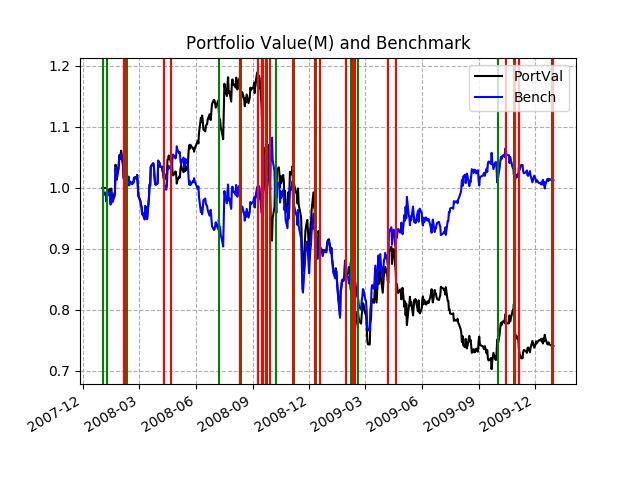
\includegraphics[scale=0.5]{isme1.png}
\caption{In-Sample Manual Strategy}
\end{subfigure}
\begin{subfigure}{.5\textwidth}
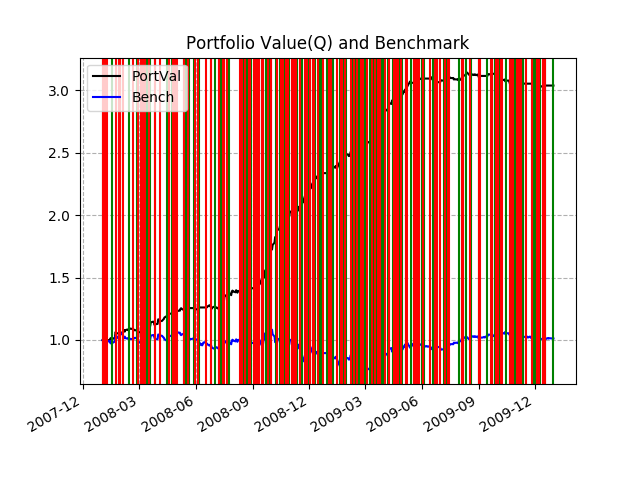
\includegraphics[scale=0.5]{isqe1.png}
\caption{In-Sample Strategy Learner}
\end{subfigure}
\end{figure}
\begin{figure}
\begin{subfigure}{.5\textwidth}
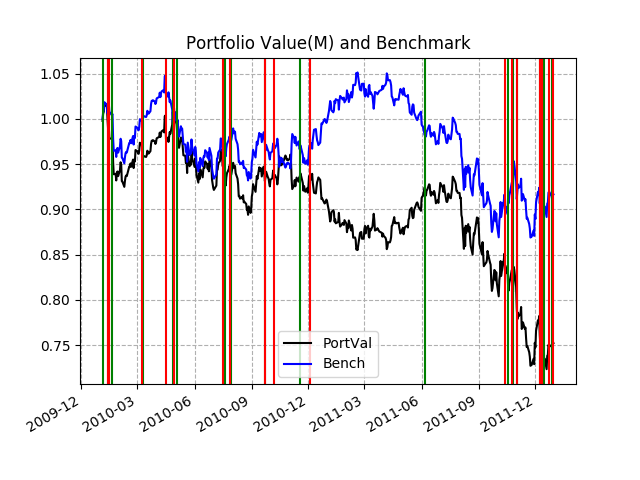
\includegraphics[scale=0.5]{osme1.png}
\caption{Out-Sample Manual Strategy}
\end{subfigure}
\begin{subfigure}{.5\textwidth}
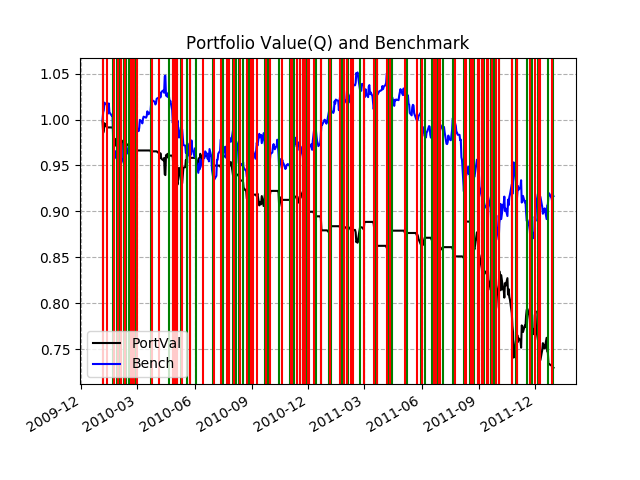
\includegraphics[scale=0.5]{osqe1.png}
\caption{Out-Sample Strategy Learner}
\end{subfigure}
\end{figure}
\text{ }\\
For the second experiment the effect of changing the value of the impact buying and selling stocks on the market was examined. The hypothesis was that with an increase in impact the total return of the trades found by the learner would drop as well as the number of trades, mostly becasue trades that had previously resulted in a positive reward might reverse. The in sample return of the learner was tested on 5 values: 0,0.0025, 0.005, 0.0075, 0.01. Surprisingly enough the learer still had a fairly high number of trades as impact increased however the effectiveness of the learner dropped considerably as it reached its highest cumulative return of 2.619 at an impact of 0.0 with 232 trades and its lowest cumulative return of 1.167 at at an impact of 0.01 with 212 trades. The impact certainly had an effect on the learner but this effect translated into shifting the dates in which the learner decided to move from long and short positions as entering and exiting was deemed more profitable at different indicators because of the increased impact, in every case the learner still utilized a high number of trades and vastly outperformed the benchmark. 

\begin{figure}
\begin{subfigure}{.5\textwidth}
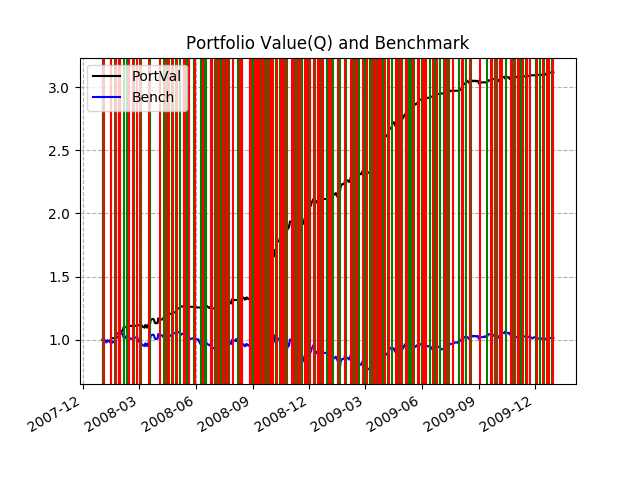
\includegraphics[scale=0.5]{ise2l.png}
\caption{In-Sample Manual Strategy}
\end{subfigure}
\begin{subfigure}{.5\textwidth}
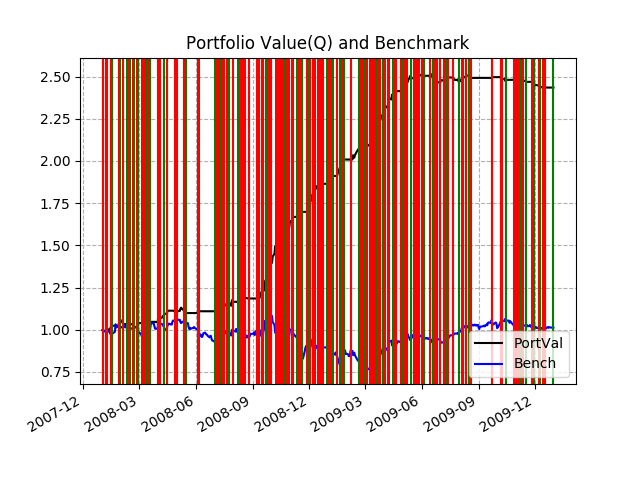
\includegraphics[scale=0.5]{ine2h.png}
\caption{In-Sample Strategy Learner}
\end{subfigure}
\end{figure}
\end{document}


